%% topic 1 spectral measures (behavioral relevance and physiological distribution on free ears)
\noindent \textbf{Vertical localization performance without molds was related to spectral information of individuals ears}\\
Participants' directional transfer functions were recorded across the vertical midline with and without earmolds. The directional transfer functions (DTFs) obtained from the left and right ear of one participant are shown in Fig. 1. To quantify spectral information available for vertical sound localization in the individual sets of DTFs, VSI \citep{trapeau_fast_2016} and spectral strength \citep{middlebrooks_individual_1999} were computed in 5 octave bands between 4 and 16 kHz. Spectral information of participants’ free ears varied among frequency bands (Kruskal-Wallis test, VSI: p = 0.009, spectral strength: p = 10e-7). The dissimilarity between DTFs across elevations (VSI) peaked in the 5.7 – 11.3 kHz band as previously reported by \citet{trapeau_fast_2016}. VSIs of participants' left and right ears were similar in this band (Spearman correlation between the VSI of left and right ears: R = 0.45, p = 0.089). Figure 2 B shows the VSIs of all participants in the 5.7 – 11.3 kHz band. Examining the variation within individual DTFs (spectral strength) revealed the highest spectral detail in the neighboring 6.7-13.5 kHz band. When joining these two bands for the analysis, VSI correlated with vertical localization accuracy (Fig 2 C) and vertical SD (free ears VSI in the 5.7 - 13.5 kHz band compared to vertical localization: RMSE: R = -0.58, p = 0.025, EG: R = 0.15, p = 0.603, SD: R = -0.58, p = 0.025). No correlation was found between behavioral metrics and spectral strength in the tested frequency bands.

%figure box A - F: Free Ears: VSI across bands, VSI LR and VSI RMSE 
\begin{figure}[h]
\begin{minipage}[t]{ \columnwidth}
	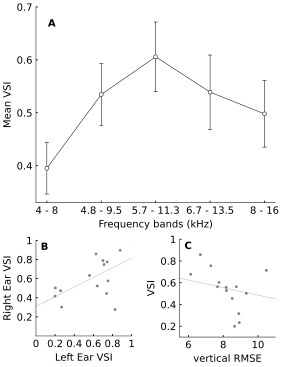
\includegraphics[width= \linewidth]{../Results/figures/fig2/fig2}
	\caption{VSI and localization performance with free ears. \textbf{A}, Variation of VSI across five octave bands between 4 and 16kHz. VSI was averaged across sets of DTFs obtained from participants' left and right ears without earmolds. VSI varies significantly and is highest in the 5.7–11.3 kHz band.  \textbf{B}, Left and right ear VSI in the 5.7-11.3 kHz band of each participant. VSIs of the left and right ears are correlated. \textbf{C}, Relation between VSI in the 5.7 – 13.5 kHz band and vertical localization accuracy.}
        \label{fig:second}
\end{minipage}
\end{figure}

%\newpage

%% topic 2 spectral effect of molds (spectral impact of molds, physiological plausibility, distribution across participants, m1m2 spectral compare)
\noindent \textbf{Earmolds reduced spectral information in the 5.7-11.3 kHz band available for vertical sound localization}\\

Application of silicone molds to the Pinnae altered spectral cues in the 4-16 kHz band. Both sets of earmolds attenuated the prominent spectral notch and the neighbouring spectral peak situated in the 5-12 kHz band (Fig. 3, A-C). Similar effects have been observed in previous studies using molds to modify spectral cues \citep{trapeau_fast_2016}\citep{wanrooij_relearning_2005}\citep{hofman_relearning_1998}. Comparing VSIs of participants' modified and free ears in the 5.7-11.3 kHz band showed that earmolds reduced the amount spectral information available for elevation discrimination (Fig 4 B, differences between VSI of free and modified ears; Free ears vs Molds 1: p = 0.0015, Free ears vs Molds 2: p = 0.0022). Both sets of earmolds led to similar levels of VSI reduction compared to participants' free ears (free ears VSI reduction caused by Mold 1 vs Mold 2: p = 0.2768).The correlation between left and right ears VSI persisted after mold insertion but was not significant for the second set of Earmolds (Molds 1: R = 0.56, p = 0.035, Molds 2: R = 0.53, p = 0.064). Figure 4 A shows participants VSIs with modified and free ears.\\

\noindent\textbf{Spectral changes occurred at similar frequencies across participants and were different for both sets of earmolds}\\

To confirm whether spectral changes occurred at similar frequencies across participants but at different frequencies in the two consecutive sets of earmolds, the probability of spectral change between free ears and earmolds was mapped for each frequency bin and elevation (Fig. 3 D-F). Spectral changes were defined as the absolute differences between DTFs measured before and after mold insertion above a given threshold. This threshold was a participant-specific measure of spectral difference across DTFs with free ears and was defined by the mean RMS difference across all combinations of DTFs (in dB) at each elevation (average across participants: 4.89 dB +/-0.15). Based on these thresholds, binary maps of spectral changes were created for each set of earmolds and participant (above-threshold changes were set to 1, all other values were set to 0). The average of these maps across participants shows the proportion of participants for which earmolds induced spectral changes above the threshold at each frequency bin and elevation.\\

%figure box A - F: DTFs of free vs modified ears and spectral change p
\begin{figure}[h]
	%\includegraphics[width=12.8cm, left]{../Results/figures/fig3/fig3}
	\includegraphics[width=12.8cm, center]{../Results/figures/fig3/fig3}
	\caption{Acoustic effect of the earmolds. \textbf{A}, Mean across participants' DTFs with free ears.
	\textbf{B-C}, Mean across participants' DTFs with modified ears. \textbf{D-E}, Probability maps showing the 		proportion of participants for which the molds induced marked changes in spectral amplitude at each elevation 		and frequency bin. \textbf{F}, Probability map showing the proportion of marked changes between the first and 		second set of molds.}
        \label{fig:third}
\end{figure}

\newpage

\noindent\textbf{Consecutive earmolds induced similar spectral changes}\\

To test whether spectral differences induced by the molds were in a similar range, VSI dissimilarities between free and modified ears were computed in the 5.7–13.5 kHz frequency band. VSI dissimilarity between participants' free ears and the first set of molds was of similar magnitude as between the first and the second set of earmolds. (Fig. 4 C,VSI dissimilarity in the 5.7–13.5 kHz band, free ears and Molds 1:  0.64 +/- 0.06 vs Molds 1 and Molds 2:  0.51 +/- 0.05: p = 0.25). The second set of earmolds induced larger spectral differences to participants' free ears than the first set (VSI dissimilarity free ears and Molds 1:  0.64 +/- 0.06 vs free ears and Molds 2: 0.8 +/- 0.06; p = 0.0005). 
\\

\noindent\textbf{Modified pinna shapes were within the physiological range}\\

To confirm that spectral changes induced by the earmolds were physiologically plausible, VSI dissimilarities between free and modified ears of each participant were compared to VSI dissimilarities between all possible pairs of participants’ free ears (Fig. 5). The overlap of distributions shows that spectral changes induced by both sets of molds were comparable in magnitude to the natural spectrum of differences between individuals’ ears.\\

% Figure box VSI across conditions, VSI dissimilarities and VSI L/R M1/M2
\begin{figure}[ht]
 	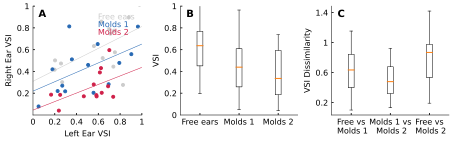
\includegraphics[width=12.8cm, left]{../Results/figures/fig4/fig4}
	\caption{caption}
        \label{fig:first}
\end{figure}

% Figure 5 overlap in VSI dissimilarities between free ears and between free ears and molds  
\begin{figure}[ht]
 	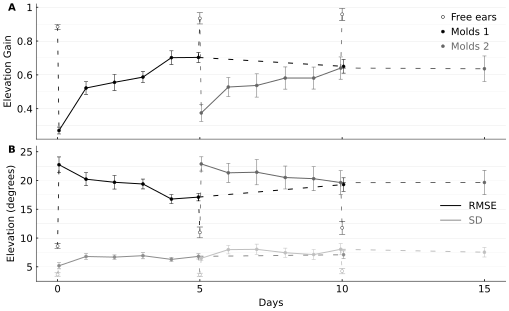
\includegraphics[width=7cm, left]{../Results/figures/fig5/fig5}
	\caption{caption}
        \label{fig:first}
\end{figure}

%% topic 3 behavior (mold impact on behavior, acoustic explanation)
\noindent \textbf{Earmolds reduced vertical localization performance}\\

Insertion of earmolds degraded vertical localization performance (see Fig. 6, days 0 and 5; one-tailed Wilcoxon signed rank test of localization performance; ears free vs earmolds 1; EG: p = 3x10-5, RMSE: p = 3x10-5, SD: p = 6x10-3 $testp =1x10^{5}$, ears free vs earmolds 2; EG: p = 5x10-4, RMSE: p = 5x10-4, SD: p = 5x10-4). On the horizontal plane, only the standard deviation of responses increased (one-tailed Wilcoxon signed rank test of performance; ears free vs earmolds 1; SD: p = 0.04, ears free vs earmolds 2: SD: p = 5x10-3). Both sets of earmolds caused a similar decrease of vertical localization performance (two-tailed Wilcoxon signed rank test, differences between free ears and earmolds 1 on day 0 vs difference between ears free and earmolds 2 on day 5; EG: p = 0.465, RMSE: p = 0.700, SD: p = 0.123).\\ %\vfill\null\columnbreak 
  
 \noindent\textbf{Effects of acoustic dissimilarity between free ears and earmolds on localization accuracy}\\

To investigate whether acoustic and behavioral effects of the earmolds were related, the VSI dissimilarity between DTFs in the 3.7 – 12.9 kHz band with and without molds was compared to the decrease in participant’s localization performance after insertion of the earmolds. A trend of increasing vertical RMSE for larger acoustic differences was found for the first set of earmolds (Fig 5 B, Spearman correlation of vertical RMSE in the first test with molds compared to free ears and VSI dissimilarity: R = 0.38, p = 0.175). The relation between acoustic differences and behavior was still visible on the last day of the adaptation period (Fig 5 C, Spearman correlation of vertical RMSE in the last test with molds compared to free ears baseline and VSI dissimilarity: R = 0.38, p = 0.185). No such trend was found for vertical localization and VSI dissimilarity between free ears and the second set of molds (Spearman correlation of vertical RMSE in the first test with molds compared to free ears baseline and VSI dissimilarity: R = - 0.07, p = 0.832). Because initial vertical localization accuracy with the second earmolds could additionally depend on acoustic similarities to the previously learned set, differences in localization performance between the final test with earmolds 1 and the initial test with the earmolds 2 were compared to the VSI dissimilarity between both molds. A trend was found of increasing vertical error with greater acoustic dissimilarity between the first and second set of earmolds (Fig 5 D, Spearman correlation of vertical RMSE in the first test with second molds compared to last test with first molds and VSI dissimilarity: R = 0.29, p = 0.385).\\
 
 % VSI dissimilarity and RMSE
 \begin{figure}[hb]
	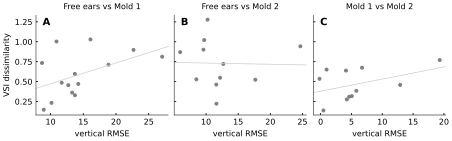
\includegraphics[width=12.8cm, left]{../Results/figures/fig6/fig6}
	\caption{caption}
        \label{fig:first}
\end{figure}

 %% topic 4 adaptation(general adaptation, rate of adaptation m1/m2, generalisability, aftereffect, persistence)
 
 \noindent\textbf{Participants consecutively adapted to two novel sets of DTFs}\\
 
Participants wore two different sets of earmolds during two consecutive 6-day adaptation periods. Adaptation was driven by multisensory experience while wearing the molds throughout the day, accompanied by five sessions of daily sensory-motor training at the lab. Vertical sound localization performance improved significantly for both sets of earmolds except for response variability (SD), which increased throughout the adaptation period (Fig 1, one-tailed Wilcoxon signed rank tests of first vs last day of molds; Earmolds 1: EG: p = 3x10-5, RMSE: p = 6x10-5, SD: p = 0.008; Earmolds 2: EG: p = 3x10-4, RMSE: p = 0.032, SD: p = 0.004). As expected, horizontal localization was not affected by adaptation to the earmolds (Fig 3 B, one-tailed Wilcoxon signed rank tests of first vs last day of molds; Earmolds 1; RMSE: p = 0.555, SD: p = 0.467; Earmolds 2; RMSE: p = 0.485, SD: p = 0.515).\\

% Learning plot
 \begin{figure}[hb]
	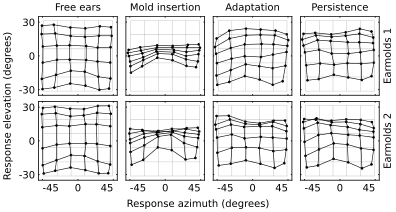
\includegraphics[width=16cm, left]{../Results/figures/fig7/fig7}
	\caption{caption}
        \label{fig:first}
\end{figure}

\noindent \textbf{No difference between rates of adaptation to first and second earmolds}\\

To investigate possible effects of metaplasticity (i.e., an effect of the previous adaptation to earmolds 1 on the subsequent adaptation to earmolds 2) the rates of adaptation to the first and second earmolds were compared. To assess the rate of adaptation across participants independent of initial acoustical disruption caused by the earmolds, the increase in vertical localization accuracy during adaptation (performance on day 0 vs day 6) was divided by the initial decrease caused by the molds. Individual adaptation rates varied continuously and did not fall into discernable groups. No difference was found between the two sets of earmolds (two-tailed Wilcoxon signed rank test of Molds 1 vs Molds 2, Reduction of vertical RMSE from day 0 to day 6 divided by initial increase; Earmolds 1: 0.66 +/- 0.06 vs Earmolds 2:  0.74 +/- 0.09, p = 0.413). Individual adaptation performance with the first set of earmolds was positively related to adaptation performance with the second set of molds, although not significant (R = 0.47, p = 0.142). No correlation was found between vertical spectral information of the earmolds in the 3.7 – 12.9 kHz band and adaptation performance.\\

\noindent\textbf{Adaptation was generalizable}\\

To rule out the possibility of participants memorizing location-specific spectral features of the training stimuli in the localization test, the test was repeated with a subset of six participants on the last day of each adaptation period using stimuli of random spectral content (USOs). The effect of USO stimuli on vertical localization error did not differ between adapted earmolds and free ears indicating that generalizable perceptual learning had taken place (Friedman test; differences in vertical RMSE between pink noise and USO localization across conditions; Ears free: -0.38 +/- 1.82, Earmolds 1: 2.5 +/- 0.46, Earmolds 2: -0.15 +/- 0.45, p = 0.135).\\

\noindent\textbf{No aftereffect on free ears localization performance after mold removal}\\

Previous studies reported the absence of an aftereffect on localization performance with free ears after adaptation to new spectral cues for sound localization (Hofman 1998, Trapeu and Schönwiesner 2015). To confirm these findings, free ears localization accuracy was measured immediately after mold removal at the end of each adaptation period. 
No aftereffect was present for elevation gain but. An increasing impact on participants’ vertical localization accuracy with their native ears was observed after each adaptation period (see Fig. 1 B, one-tailed Wilcoxon signed rank test, vertical RMSE; free ears baseline vs free ears day 5: p = 0.002, free ears baseline vs free ears day 10: p = 6x10-4). \\

% Learning plot
 \begin{figure}[hb]
	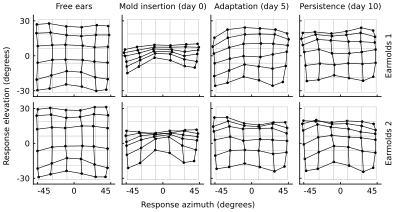
\includegraphics[width=16cm, left]{../Results/figures/fig8/fig8}
	\caption{caption}
        \label{fig:first}
\end{figure}

